\documentclass[a4paper,11pt]{article}
\usepackage[utf8]{inputenc}
\usepackage{amsmath}
\usepackage{amsfonts}
\usepackage{amssymb}
\usepackage[hidelinks]{hyperref}
\usepackage{geometry}
\geometry{margin=1in}
\usepackage{enumitem}
\usepackage{xcolor}
\usepackage{tikz}

\newcommand{\hint}[1]{\textit{\color{gray!70!black}Hint: #1}}
\newcommand{\idea}{\vspace{4pt}\begin{itemize}[leftmargin=1.2em]\item[--] \end{itemize}\vspace{-8pt}}

\title{CSCib Lab notes}
\author{}
\date{}

\begin{document}
\maketitle

\section*{2 -- Plant description}

\subsection*{Q1 -- Analyzing the problem}
\label{sec:q1}

\subsubsection*{Why is achieving this control objective nontrivial?}


\vspace{6pt}

\paragraph{System.}
The plant is a DC servo motor (with gearbox) driving a thin flexible beam clamped to its output
shaft, the Quanser \emph{Rotary Flexible Link} module (FLEXGAGE) on an SRV02 base. Its state vector has four physical states:
$$x = [\theta \ \ \omega{=}\dot\theta \ \ \alpha \ \ \beta{=}\dot\alpha]^T.$$
Our guide combines $\theta,\alpha$ into a single output $y=\theta+\alpha$ for SISO identification
in Part~I.
\paragraph{Why four states, hence four poles?}
Each state represents an independent way in which energy can be stored in the system: the motor's kinetic energy is captured by $\omega$, the shaft position by $\theta$, the link's elastic energy by $\alpha$, and the link tip's kinetic energy by $\beta$. Since there are four independent states, the system is fourth order and therefore has four poles. \textbf{To place these poles independently, we need four independent feedback gains}.


\paragraph{State equations and their physical meaning.}
\begin{itemize}
  \item $\dot\theta = \omega$:  the shaft angle is the accumulated history of the shaft speed.
  \item $\dot\omega = -a\omega + bu$: the motor speed responds to the voltage $u$ with a
  first-order lag set by the shaft's inertia and its friction/back-EMF damping.
  \item $\dot\alpha = \beta$: the deflection angle is the accumulated history of the deflection
  rate.
  \item $\dot\beta = -\omega_n^2\alpha - 2\zeta\omega_n\beta - \dot\omega$: the link vibrates like
  a lightly-damped spring-mass system (stiffness $K_s$, damping $B_l$), excited by the base's own angular acceleration.
\end{itemize}

\paragraph{(a) Feasibility of a voltage lookup table.}
No. Since $\dot\theta=\omega$, the relation between $u$ and $\theta$ contains a pure integrator, meaning that there is no restoring effect that naturally brings the shaft to a specific position. In practice, stopping at a target angle would require knowing exactly how much voltage to apply and exactly when to stop applying it. Even then, such a lookup table would only work under very repeatable conditions, since effects such as friction, gearbox backlash, and the link's oscillations can change from one run to another. A closed-loop controller is therefore needed to correct the motion in real time.

\paragraph{(b) Result of a constant voltage.}
This is simply the extreme case of (a). If $u=\text{const}\neq0$, the motor reaches a nonzero steady-state speed, so $\omega\to\text{const}\neq0$. As a result, $\theta$ keeps increasing and never settles at a fixed value. \textbf{This is exactly the behaviour we would expect from the integrator in the position dynamics.}

\paragraph{(c) Would a single proportional gain work?}
The main problem is not steady-state error. Since $G(0)=\infty$ due to the integrator, the closed-loop DC gain satisfies $T(0)\to1$ for any stabilizing $K$. Therefore, once closed-loop stability has been established separately, a step reference can be tracked with zero steady-state error.

The real issue is performance. A single gain has to control both the speed of the position response and the damping of the lightly damped complex poles associated with the link dynamics. If $K$ is too small, the link vibrations remain poorly damped. If $K$ is increased to obtain a faster position response, the same poles can move towards the imaginary axis and eventually lead to instability. This leaves only a limited and potentially fragile range of gains. A full-state feedback controller is therefore a much more effective solution, since it allows these different objectives to be controlled more independently.


\paragraph{(d) Approximate open-loop pole distribution.}
Three physical origins, four poles:
\begin{itemize}
  \item $s=0$ -- the shaft-position integrator, see (a)/(b).
  \item $s=-a$ -- the motor's own electromechanical time constant.
  \item $s=-\zeta\omega_n \pm j\omega_n\sqrt{1-\zeta^2}$, small $\zeta$ -- the link's
  lightly-damped vibration mode, close to the imaginary axis.
\end{itemize}

\begin{figure}[h]
\centering
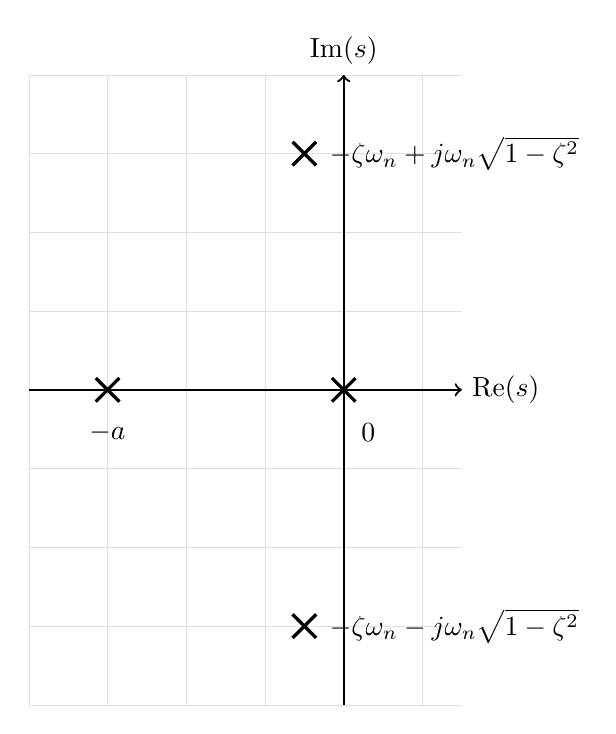
\begin{tikzpicture}
  \draw[help lines, color=gray!25] (-4,-4) grid (1.5,4);
  \draw[->, thick] (-4,0) -- (1.5,0) node[right] {$\mathrm{Re}(s)$};
  \draw[->, thick] (0,-4) -- (0,4) node[above] {$\mathrm{Im}(s)$};

  \draw[very thick] (-0.15,-0.15) -- (0.15,0.15);
  \draw[very thick] (-0.15,0.15) -- (0.15,-0.15);
  \node[below right] at (0.1,-0.3) {$0$};

  \draw[very thick] (-3.15,-0.15) -- (-2.85,0.15);
  \draw[very thick] (-3.15,0.15) -- (-2.85,-0.15);
  \node[below] at (-3,-0.3) {$-a$};

  \draw[very thick] (-0.65,2.85) -- (-0.35,3.15);
  \draw[very thick] (-0.65,3.15) -- (-0.35,2.85);
  \node[right] at (-0.3,3) {$-\zeta\omega_n + j\omega_n\sqrt{1-\zeta^2}$};

  \draw[very thick] (-0.65,-3.15) -- (-0.35,-2.85);
  \draw[very thick] (-0.65,-2.85) -- (-0.35,-3.15);
  \node[right] at (-0.3,-3) {$-\zeta\omega_n - j\omega_n\sqrt{1-\zeta^2}$};
\end{tikzpicture}
\caption{Qualitative open-loop pole map (illustrative, not to scale).}
\label{fig:q1-poles}
\end{figure}

Consistent with the identification workflow in the reference guide.


\subsection*{2.2 -- Flexible bar deflection transducer}
Calibrating $K_e$ matters because the strain gauge is slightly nonlinear and drifts a bit between
trials, so it must be fitted by least squares rather than assumed. Any error in $K_e$ becomes a
systematic scaling error in $\alpha$, in the combined output $y=\theta+\alpha$, and in the
$|\alpha|\le10^\circ$ safety limit.


\subsection*{2.3 -- Shaft angle transducer}
Calibrating $K_p$ matters for the same reason: it converts the potentiometer voltage into the
real shaft angle $\theta$ used in $y=\theta+\alpha$ and in every model/controller built
afterwards -- an error here silently rescales the whole plant model.


\end{document}
